\begin{flushright} {\tiny {\color{gray} python\_codes/fieldstone\_115/text.tex}} \end{flushright}

\lstinputlisting[language=bash,basicstyle=\small]{python_codes/fieldstone_115/keywords}

\begin{center}
\fbox{\textbf{\huge \color{teal} P}}
Codes at \url{https://github.com/cedrict/fieldstone/tree/master/python_codes/fieldstone_115}
\end{center}

\par\noindent\rule{\textwidth}{0.4pt}

%%%%%%%%%%%%%%%%%%%%%%%%%%%%%%%%%%%%%%%%%%%%%%%%%%%%%%%%%%%%%%%%%%%%%%%%%%%%%%%%%%%%%%%%%%%%%%


When it comes to the stabilisation of the $Q_1\times P_0$ elements, 
we have seen in Section~\ref{ss:pairq1p0stab} that mulitple types co-exist
and that a tuning parameter $\epsilon$ plays a role. 
Despite the published literature on the topic, the following questions remain:

- how to deal with vicosity contrasts ? 

- which stab is best for real life geodynamics ? 

- how to deal with not square mesh ?

- how to choose the $\epsilon$ value ?

- look at buoyancy driven flows. lith pressure!

WTF is macro-element stab?!!


%====================================================================================
\subsection{Donea \& Huerta manufactured solution}


\begin{center}
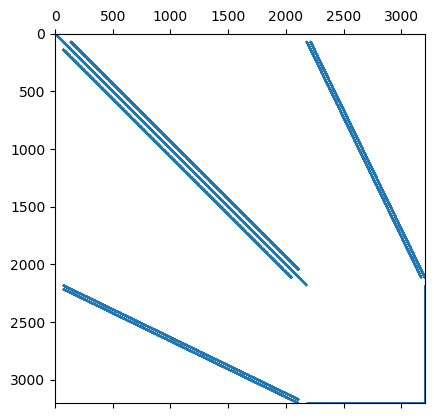
\includegraphics[width=6cm]{python_codes/fieldstone_115/results/dh/nostab/matrix}
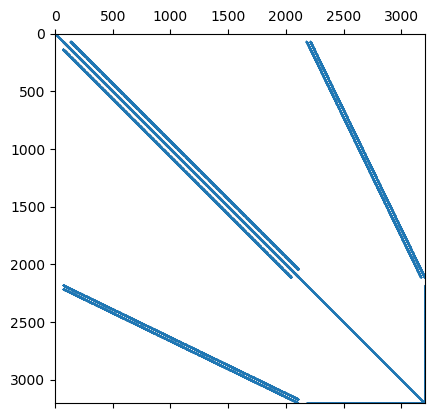
\includegraphics[width=6cm]{python_codes/fieldstone_115/results/dh/penalty/matrix}
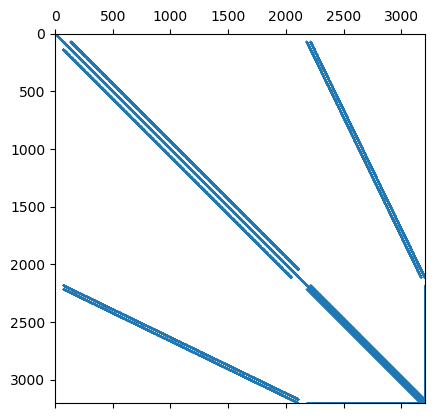
\includegraphics[width=6cm]{python_codes/fieldstone_115/results/dh/global/matrix}
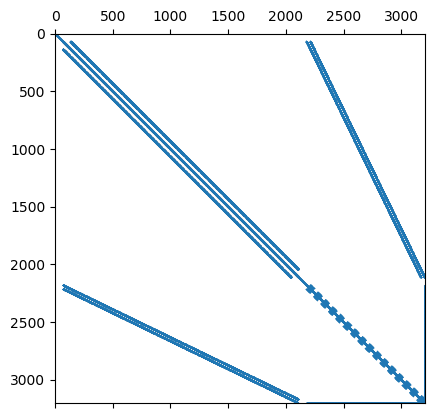
\includegraphics[width=6cm]{python_codes/fieldstone_115/results/dh/local/matrix}\\
{\captionfont 32x32. From left to right: parsity pattern of the FEM matric for 
no stabilisation, penalty, global, local.}
\end{center}

We find that all three stabilisation $\C$ matrices are enough to suppress the chequerboard mode:
\begin{center}
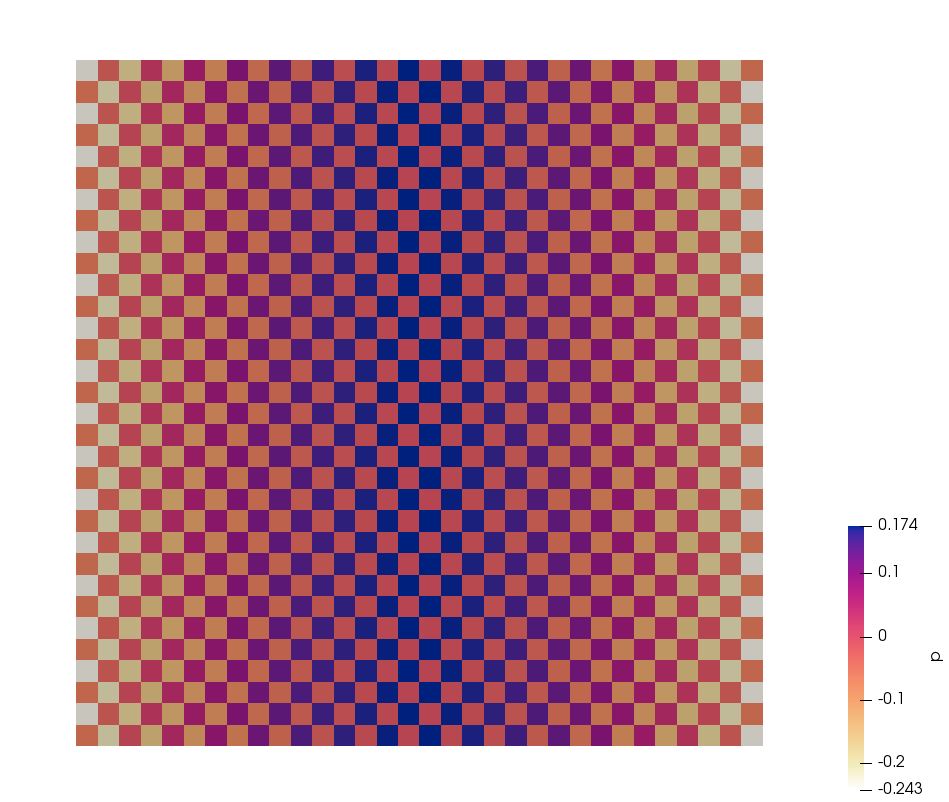
\includegraphics[width=4cm]{python_codes/fieldstone_115/results/dh/nostab/press}
\includegraphics[width=4cm]{python_codes/fieldstone_115/results/dh/penalty/press}
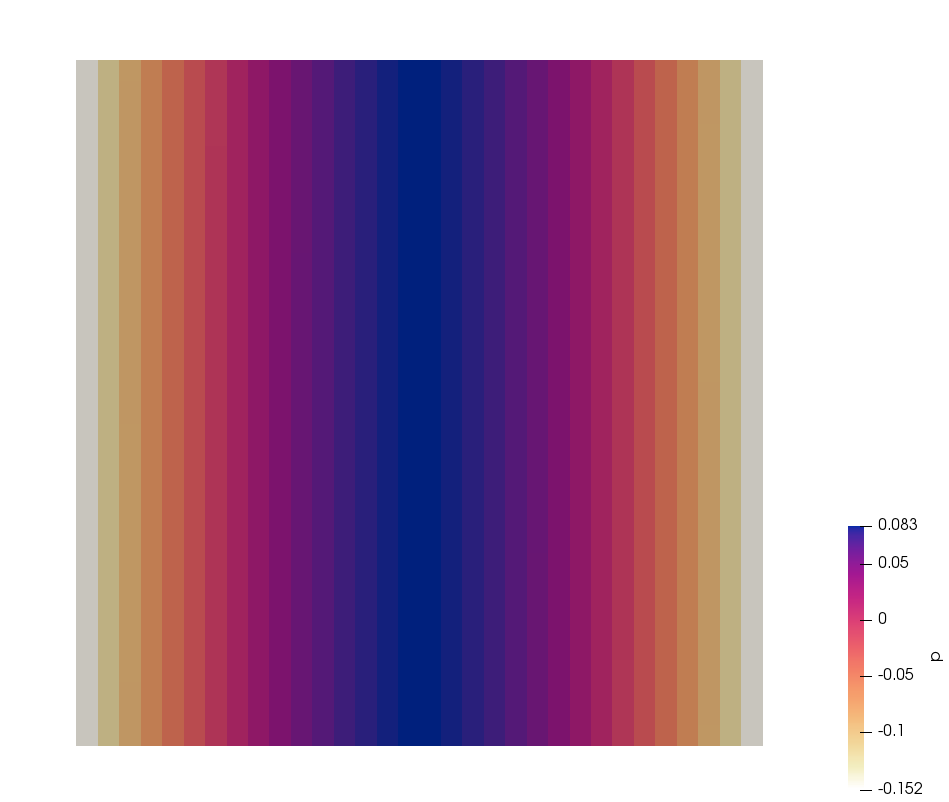
\includegraphics[width=4cm]{python_codes/fieldstone_115/results/dh/global/press}
\includegraphics[width=4cm]{python_codes/fieldstone_115/results/dh/local/press}\\
{\captionfont 32x32. From eft to right: no stabilisation, penalty, global, local. $\epsilon=10^{-10}$}
\end{center}

We can now explore the influence of the stabilisation parameter $\epsilon$. Obviously, 
if too low it won't have any effect as the $\C$ matrix then tends to zero. If too high,
then we expect it to perturb the solution too much. 
The pressure field is shown in the following figure for various values of $\epsilon$, 

and no pressure normalisation is implemented at all. We find that not only the 
penalty stabilisation removes the chequerboard mode but it also automatically 
normalises the pressure...?  

\begin{center}
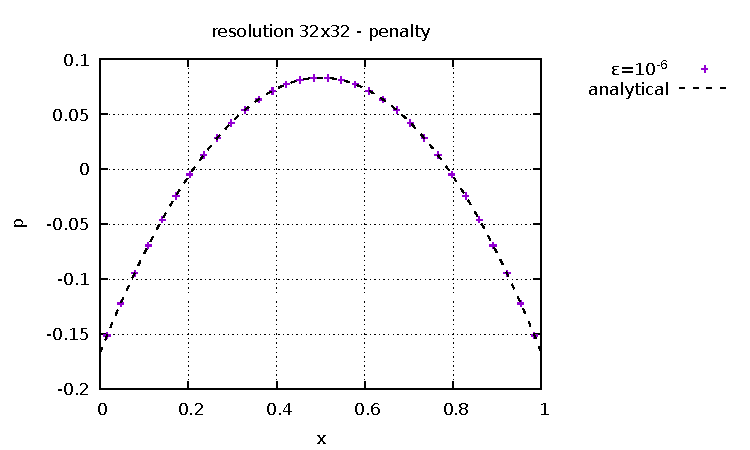
\includegraphics[width=5.7cm]{python_codes/fieldstone_115/results/dh/pressure_penalty.pdf}
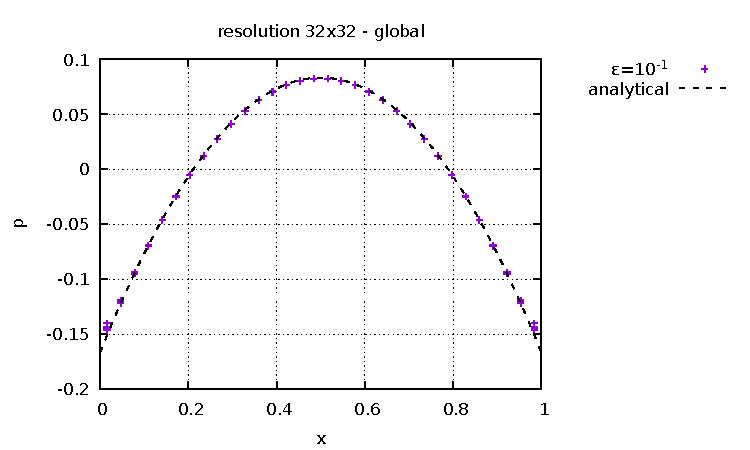
\includegraphics[width=5.7cm]{python_codes/fieldstone_115/results/dh/pressure_global.pdf}
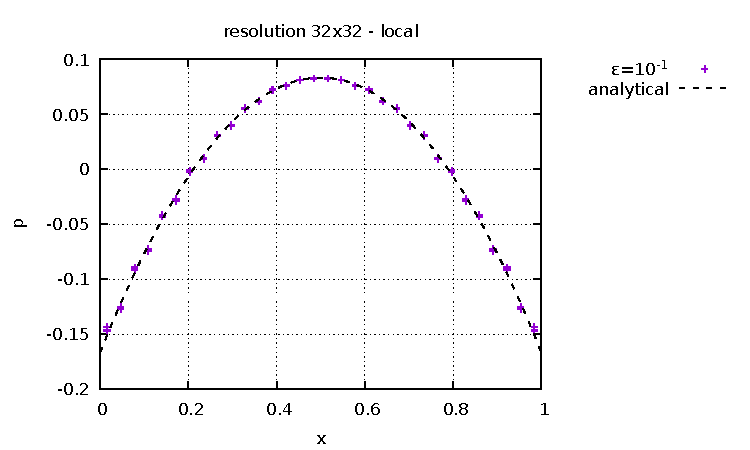
\includegraphics[width=5.7cm]{python_codes/fieldstone_115/results/dh/pressure_local.pdf}\\
{\captionfont 32x32. influence of $\epsilon$ parameter} 
\end{center}

Let us now turn to the error convergence rates after carrying out a pressure normalisation 
as a postprocessor:
\begin{center}
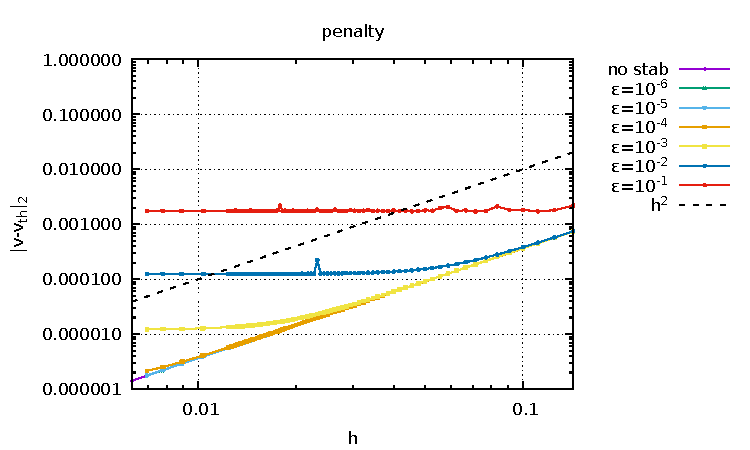
\includegraphics[width=5.7cm]{python_codes/fieldstone_115/results/dh/errorsV_penalty.pdf}
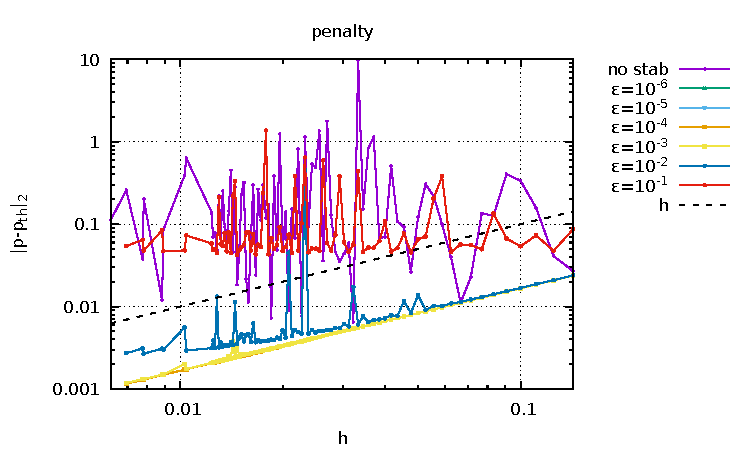
\includegraphics[width=5.7cm]{python_codes/fieldstone_115/results/dh/errorsP_penalty.pdf}
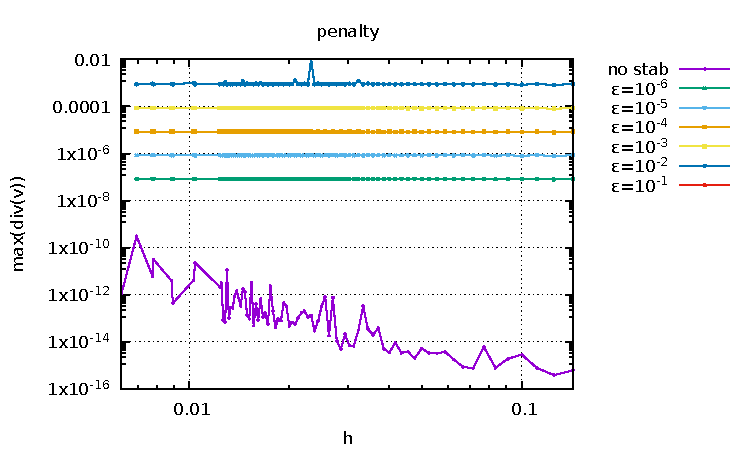
\includegraphics[width=5.7cm]{python_codes/fieldstone_115/results/dh/divv_penalty.pdf}\\
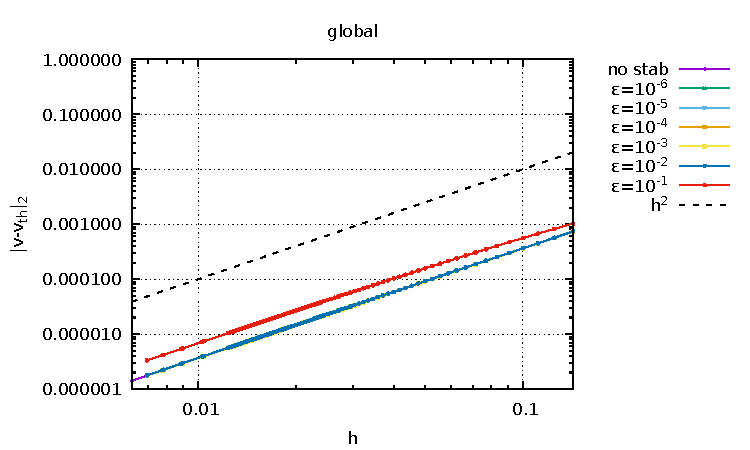
\includegraphics[width=5.7cm]{python_codes/fieldstone_115/results/dh/errorsV_global.pdf}
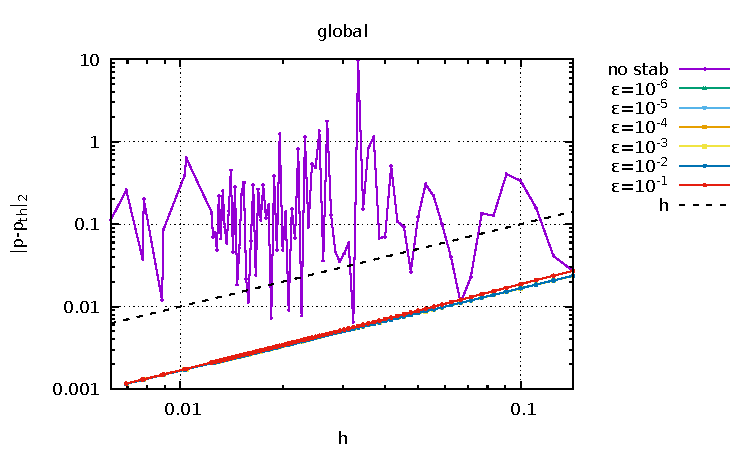
\includegraphics[width=5.7cm]{python_codes/fieldstone_115/results/dh/errorsP_global.pdf}
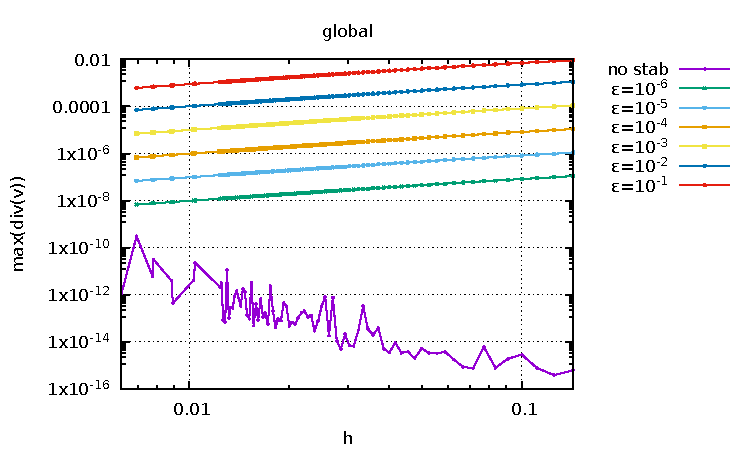
\includegraphics[width=5.7cm]{python_codes/fieldstone_115/results/dh/divv_global.pdf}\\
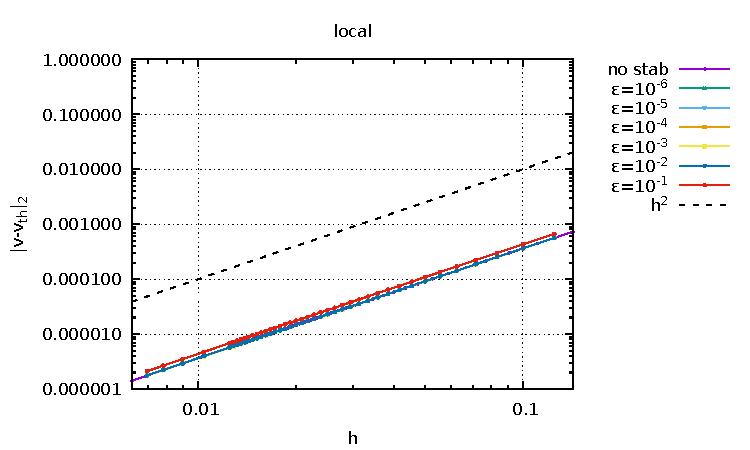
\includegraphics[width=5.7cm]{python_codes/fieldstone_115/results/dh/errorsV_local.pdf}
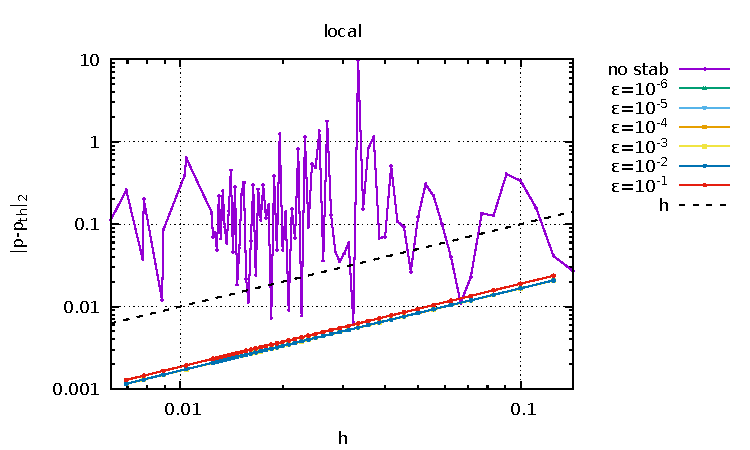
\includegraphics[width=5.7cm]{python_codes/fieldstone_115/results/dh/errorsP_local.pdf}
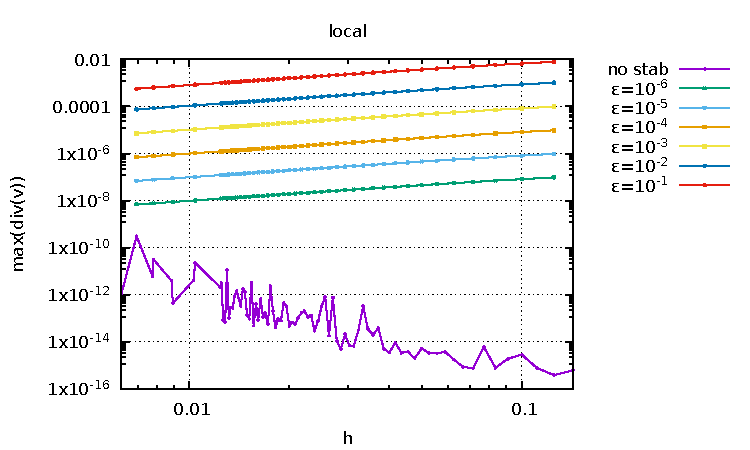
\includegraphics[width=5.7cm]{python_codes/fieldstone_115/results/dh/divv_local.pdf}\\
{\captionfont Velocity and pressure errors as a function of the element size for meshes 6x6 to 128x128}
\end{center}
We find that the error convergence rate for velocity is always quadratic as expected, 
while the error convergence for pressure becomes monotonous and linear as expected for $\epsilon\ge >10^{-13}$.
We also see that when $\epsilon$ becomes too large then the velocity error rate increases at higher resolutions.


I should monitor the condition number of the matrix...

\newpage
%====================================================================================
\subsection{The aquarium}

The domain is still a unit square. Boundary conditions are no slip on all sides. 
Density and viscosity are set to 1. Gravity is vertical with $\vec{g}=-\vec{e}_y$.
The analytical velocity is obviously $\vec\upnu=\vec{0}$ and the analytical pressure
is $p(x,y)=0.5-y$ (which fulfils $\int_\Omega p dV=0$).

Because the analytical velocity field is a constant, it can be represented exactly 
by bi-linear functions so we expect the velocity error to be at machine precision
independently of the resolution. However, because of the presence of the stabilisation
term, we find in the penalty case that it is proportional to $\epsilon$ and 
in the global and local cases that it converges quadratically.

The analytical pressure field, on the other hand is a linear polynomial which cannot 
be represented exactly by a set of discontinuous $C^0$ functions. We then expect and receover 
a linear convergence.


\begin{center}
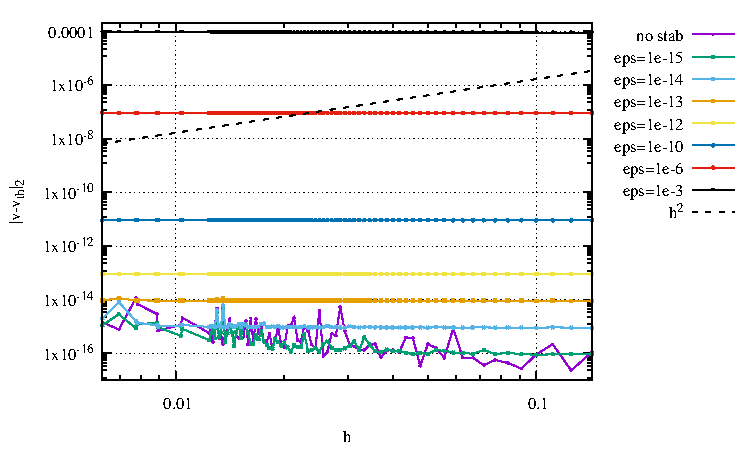
\includegraphics[width=5.7cm]{python_codes/fieldstone_115/results/aquarium/errorsV_penalty.pdf}
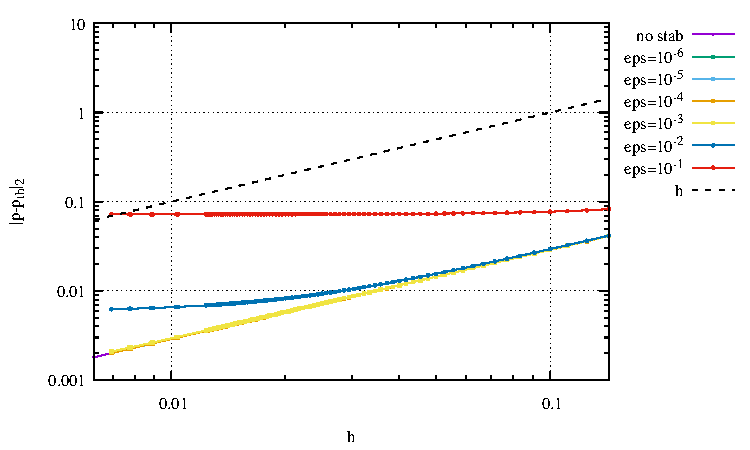
\includegraphics[width=5.7cm]{python_codes/fieldstone_115/results/aquarium/errorsP_penalty.pdf}
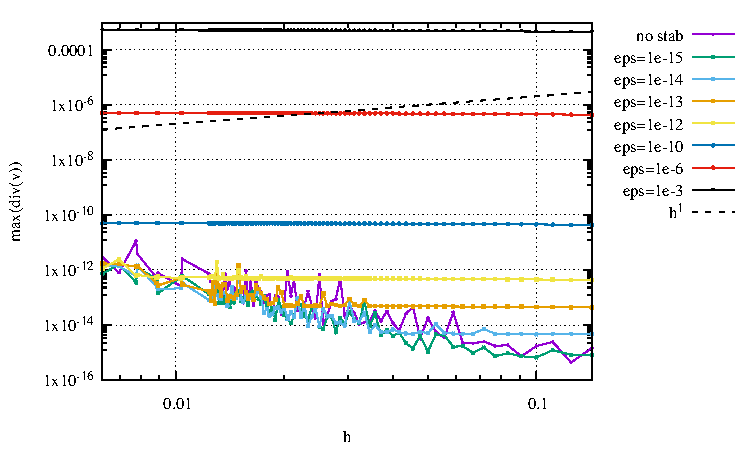
\includegraphics[width=5.7cm]{python_codes/fieldstone_115/results/aquarium/divv_penalty.pdf}\\
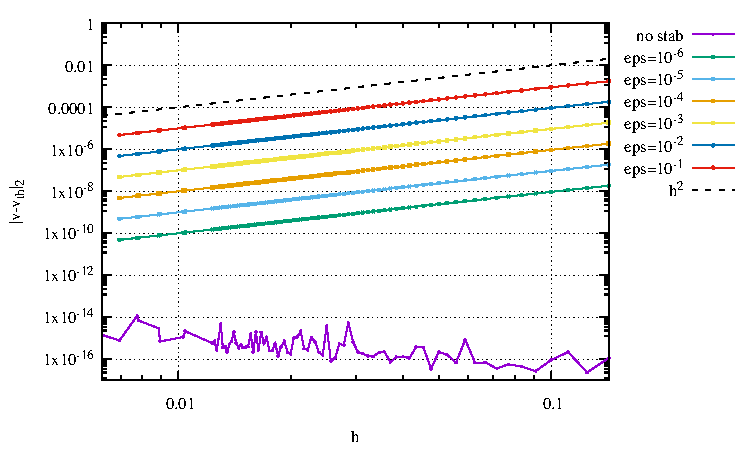
\includegraphics[width=5.7cm]{python_codes/fieldstone_115/results/aquarium/errorsV_global.pdf}
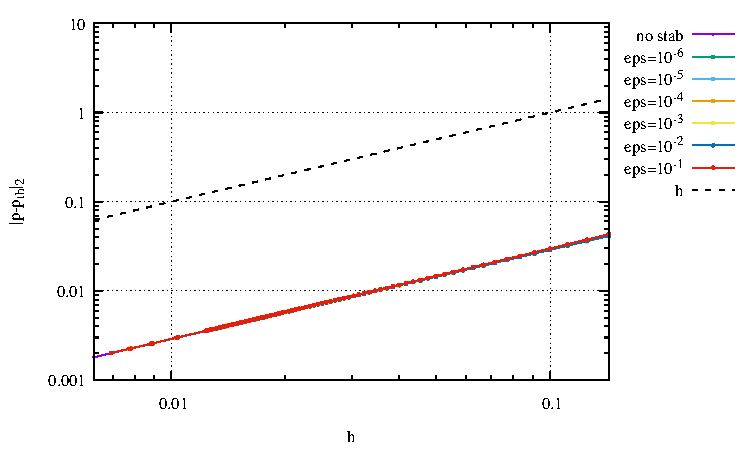
\includegraphics[width=5.7cm]{python_codes/fieldstone_115/results/aquarium/errorsP_global.pdf}
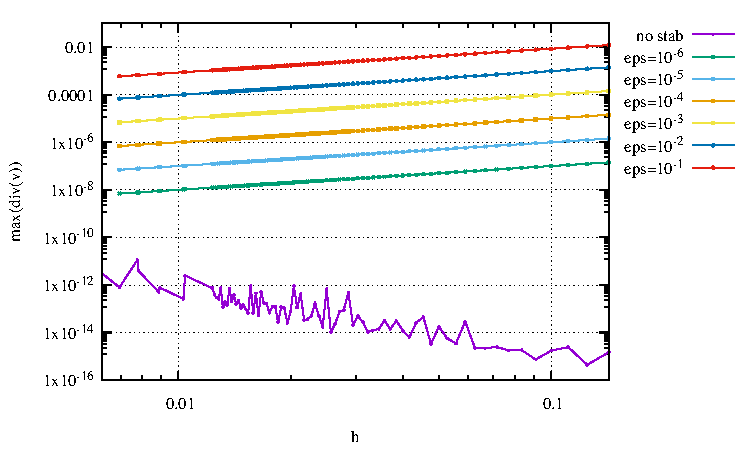
\includegraphics[width=5.7cm]{python_codes/fieldstone_115/results/aquarium/divv_global.pdf}\\
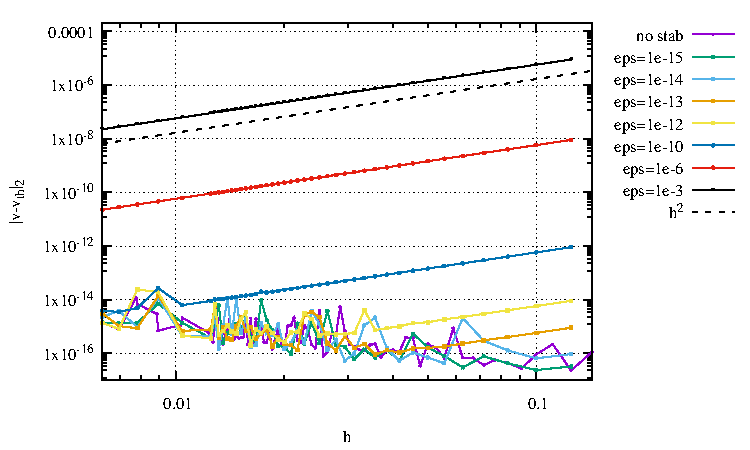
\includegraphics[width=5.7cm]{python_codes/fieldstone_115/results/aquarium/errorsV_local.pdf}
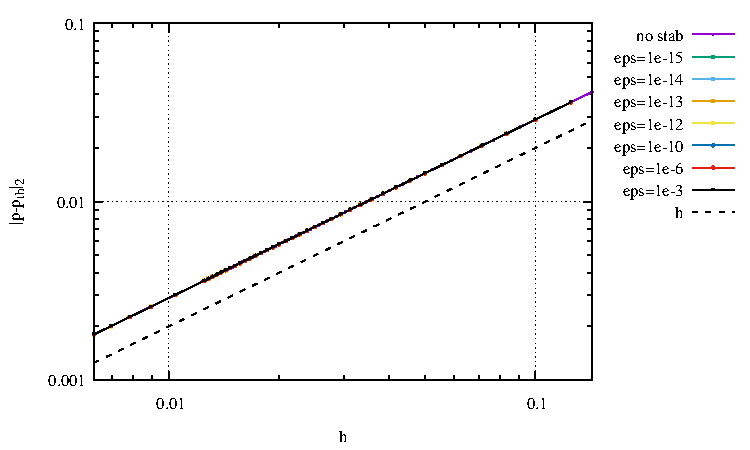
\includegraphics[width=5.7cm]{python_codes/fieldstone_115/results/aquarium/errorsP_local.pdf}
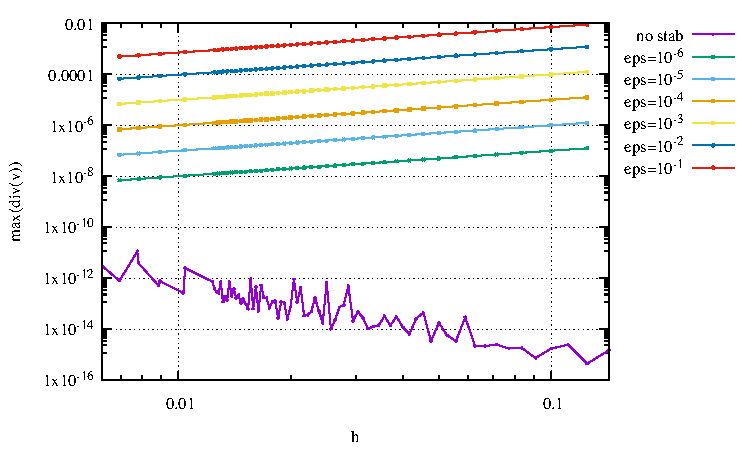
\includegraphics[width=5.7cm]{python_codes/fieldstone_115/results/aquarium/divv_local.pdf}\\
{\captionfont Left to right: vel error, press error, and max(div(v)). top to bottom: 
penalty, global, local.}
\end{center}


\newpage
%====================================================================================
\subsection{Lid driven cavity}

see elefant





